\documentclass{article}

\usepackage{tikz} 
\usetikzlibrary{automata, positioning, arrows} 

\usepackage{amsthm}
\usepackage{amsfonts}
\usepackage{amsmath}
\usepackage{amssymb}
\usepackage{fullpage}
\usepackage{color}
\usepackage{parskip}
\usepackage{hyperref}
  \hypersetup{
    colorlinks = true,
    urlcolor = blue,       % color of external links using \href
    linkcolor= blue,       % color of internal links 
    citecolor= blue,       % color of links to bibliography
    filecolor= blue,        % color of file links
    }
    
\usepackage{graphicx}
\usepackage{float}
\graphicspath{{.}{report/}}  % find images in current dir or report/ (when compiling from project root)
\usepackage{ifthen}
\usepackage{listings}
\usepackage[utf8]{inputenc}                                                    
\usepackage[T1]{fontenc}                                                       

% Turing machine tape blank symbol
\newcommand{\blank}{\sqcup}

\definecolor{dkgreen}{rgb}{0,0.6,0}
\definecolor{gray}{rgb}{0.5,0.5,0.5}
\definecolor{mauve}{rgb}{0.58,0,0.82}

\lstset{frame=tb,
  language=haskell,
  aboveskip=3mm,
  belowskip=3mm,
  showstringspaces=false,
  columns=flexible,
  basicstyle={\small\ttfamily},
  numbers=none,
  numberstyle=\tiny\color{gray},
  keywordstyle=\color{blue},
  commentstyle=\color{dkgreen},
  stringstyle=\color{mauve},
  breaklines=true,
  breakatwhitespace=true,
  tabsize=3
}

\newtheoremstyle{theorem}
  {\topsep}   % ABOVESPACE
  {\topsep}   % BELOWSPACE
  {\itshape\/}  % BODYFONT
  {0pt}       % INDENT (empty value is the same as 0pt)
  {\bfseries} % HEADFONT
  {.}         % HEADPUNCT
  {5pt plus 1pt minus 1pt} % HEADSPACE
  {}          % CUSTOM-HEAD-SPEC
\theoremstyle{theorem} 
   \newtheorem{theorem}{Theorem}[section]
   \newtheorem{corollary}[theorem]{Corollary}
   \newtheorem{lemma}[theorem]{Lemma}
   \newtheorem{proposition}[theorem]{Proposition}
\theoremstyle{definition}
   \newtheorem{definition}[theorem]{Definition}
   \newtheorem{example}[theorem]{Example}
\theoremstyle{remark}    
  \newtheorem{remark}[theorem]{Remark}

\title{CPSC-406 Report}
\author{Sami Hammoud  \\ Chapman University}

\date{\today} 

\begin{document}

\maketitle

\begin{abstract}
\end{abstract}

\setcounter{tocdepth}{3}
\tableofcontents

\section{Introduction}\label{intro}

\section{Week by Week}\label{homework}

\subsection{Week 1}

\subsubsection*{Exercise 1}
Consider the following DFAs $\mathcal{A}_1$ and $\mathcal{A}_2$. Complete the following table with all 8 possible strings of length 3 over $\{a,b\}$ (columns: Accepted by $\mathcal{A}_1$? and Accepted by $\mathcal{A}_2$?).

\paragraph{Answer to Exercise 1.1.}
Here is my completed table (words of length~3 over $\{a,b\}$):

\begin{center}
\begin{tabular}{|c|c|c|}
  \hline
  word & Accepted by $\mathcal{A}_1$? & Accepted by $\mathcal{A}_2$? \\
  \hline
  $aaa$ & No  & Yes \\
  $aab$ & Yes & No  \\
  $aba$ & No  & No  \\
  $abb$ & No  & No  \\
  $baa$ & No  & Yes \\
  $bab$ & No  & No  \\
  $bba$ & No  & No  \\
  $bbb$ & No  & No  \\
  \hline
\end{tabular}
\end{center}

\subsubsection*{Exercise 1.2}
Describe the languages $L(\mathcal{A}_k)$ accepted by $\mathcal{A}_k$ for $k = 1, 2$.

\paragraph{Answer to Exercise 1.2.}
For $k = 1$, $L(\mathcal{A}_1)$ is just the single word \emph{aab}.  
For $k = 2$, $L(\mathcal{A}_2)$ is all words over $\{a,b\}$ that end in \emph{at least two $a$'s in a row} (so the last two symbols are $aa$).

\subsubsection*{Exercise 2 (Designing DFAs)}
Design DFAs whose accepted languages are given as follows:
\begin{enumerate}
  \item All the words that end with $ab$
  \item All the words that contain $aba$
  \item All the words that contain an odd number of $a$'s and an odd number of $b$'s
  \item All the words that contain an even number of $a$'s and an odd number of $b$'s
  \item All the words such that any three consecutive characters contain at least one $a$
  \item All the words that contain $bbb$
\end{enumerate}
\textbf{What do you notice when comparing the various automata?}

\paragraph{Answers for Exercise 2.}

\paragraph{(1) Words that end with $ab$.}
I use three states that remember the last one or two symbols. The DFA is:

\begin{figure}[H]
  \centering
  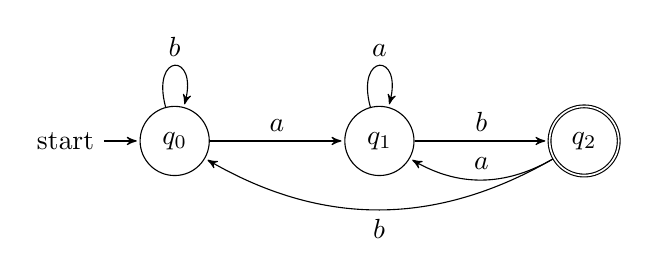
\begin{tikzpicture}[>=stealth',shorten >=1pt,node distance=2.6cm,on grid,auto]
    \node[state,initial] (q0) {$q_0$};
    \node[state] (q1) [right=of q0] {$q_1$};
    \node[state,accepting] (q2) [right=of q1] {$q_2$};
    \path[->]
      (q0) edge[loop above] node {$b$} ()
           edge node {$a$} (q1)
      (q1) edge[loop above] node {$a$} ()
           edge node {$b$} (q2)
      (q2) edge[bend left] node[above] {$a$} (q1)
           edge[bend left] node[below] {$b$} (q0);
  \end{tikzpicture}
  \caption{DFA for all words that end with $ab$.}
  \label{fig:week1-endab}
\end{figure}

\paragraph{(2) Words that contain $aba$.}
Here I track how much of the pattern $aba$ I have just seen as a suffix.

\begin{figure}[H]
  \centering
  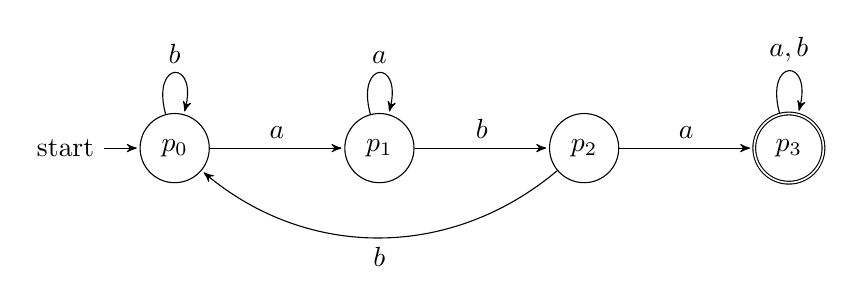
\begin{tikzpicture}[>=stealth',shorten >=1pt,node distance=2.6cm,on grid,auto]
    \node[state,initial] (p0) {$p_0$};
    \node[state] (p1) [right=of p0] {$p_1$};
    \node[state] (p2) [right=of p1] {$p_2$};
    \node[state,accepting] (p3) [right=of p2] {$p_3$};
    \path[->]
      (p0) edge[loop above] node {$b$} ()
           edge node {$a$} (p1)
      (p1) edge[loop above] node {$a$} ()
           edge node {$b$} (p2)
      (p2) edge node {$a$} (p3)
           edge[bend left=40] node[below] {$b$} (p0)
      (p3) edge[loop above] node {$a,b$} ();
  \end{tikzpicture}
  \caption{DFA for all words that contain $aba$ as a substring.}
  \label{fig:week1-contains-aba}
\end{figure}

\paragraph{(3) Odd number of $a$'s and odd number of $b$'s.}
For this and the next language I use the same 4-state parity automaton, but choose different accepting states. The four states remember the parity (even/odd) of the number of $a$'s and $b$'s seen so far.

\begin{figure}[H]
  \centering
  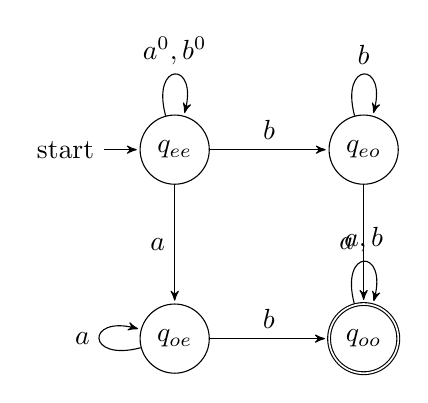
\begin{tikzpicture}[>=stealth',shorten >=1pt,node distance=2.4cm,on grid,auto]
    \node[state,initial] (ee) {$q_{ee}$};
    \node[state] (eo) [right=of ee] {$q_{eo}$};
    \node[state] (oe) [below=of ee] {$q_{oe}$};
    \node[state,accepting] (oo) [right=of oe] {$q_{oo}$};
    \path[->]
      (ee) edge[loop above] node {$a^0,b^0$} ()
           edge node {$b$} (eo)
           edge node[left] {$a$} (oe)
      (eo) edge[loop above] node {$b$} ()
           edge node[left] {$a$} (oo)
      (oe) edge[loop left] node {$a$} ()
           edge node {$b$} (oo)
      (oo) edge[loop above] node {$a,b$} ();
  \end{tikzpicture}
  \caption{Parity DFA: state $q_{xy}$ means $x$-parity for $a$'s and $y$-parity for $b$'s. For language (3) we accept $q_{oo}$ (odd $a$'s and odd $b$'s).}
  \label{fig:week1-parity}
\end{figure}

\paragraph{(4) Even number of $a$'s and odd number of $b$'s.}
Using the same parity DFA in Figure~\ref{fig:week1-parity}, this time the accepting state is $q_{eo}$ (even $a$'s, odd $b$'s) instead of $q_{oo}$.

\paragraph{(5) Any three consecutive characters contain at least one $a$.}
This is the same as saying that we never see $bbb$ as a substring. I track runs of consecutive $b$'s up to length~3; hitting three $b$'s in a row moves to a dead (rejecting) state.

\begin{figure}[H]
  \centering
  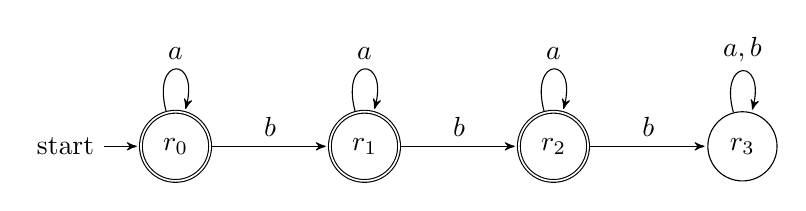
\begin{tikzpicture}[>=stealth',shorten >=1pt,node distance=2.4cm,on grid,auto]
    \node[state,initial,accepting] (r0) {$r_0$};
    \node[state,accepting] (r1) [right=of r0] {$r_1$};
    \node[state,accepting] (r2) [right=of r1] {$r_2$};
    \node[state] (r3) [right=of r2] {$r_3$};
    \path[->]
      (r0) edge[loop above] node {$a$} ()
           edge node {$b$} (r1)
      (r1) edge[loop above] node {$a$} ()
           edge node {$b$} (r2)
      (r2) edge[loop above] node {$a$} ()
           edge node {$b$} (r3)
      (r3) edge[loop above] node {$a,b$} ();
  \end{tikzpicture}
  \caption{DFA that forbids $bbb$; states $r_0,r_1,r_2$ are accepting, $r_3$ is a dead state reached after three $b$'s in a row.}
  \label{fig:week1-nobbb}
\end{figure}

\paragraph{(6) Words that contain $bbb$.}
I reuse the same transition structure as in Figure~\ref{fig:week1-nobbb}, but now $r_3$ is the \emph{only} accepting state (once we have seen three consecutive $b$'s we stay in an accepting sink).

\paragraph{What I notice.}
Several of these automata reuse the same underlying structure but just change which states are accepting (for example (3) vs.\ (4), and (5) vs.\ (6)). In other words, a lot of the ``different'' languages here really come from the same core DFA with a different choice of final states.

\subsubsection*{Question}
How might you combine the languages $L(\mathcal{A}_1)$ and $L(\mathcal{A}_2)$ from Exercise 1 using set operations (union, intersection, complement)? Could you represent the logic with boolean logic exclusively?

\subsection{Week 2: Operations on Automata}\label{sec:week2}

\subsubsection*{Product automata}



\subsubsection*{Exercise 1 (Product automata)}

Consider the following automata $\mathcal{A}^{(1)}$ and $\mathcal{A}^{(2)}$.

\begin{figure}[ht]
  \centering
  \IfFileExists{A1hw2.png}{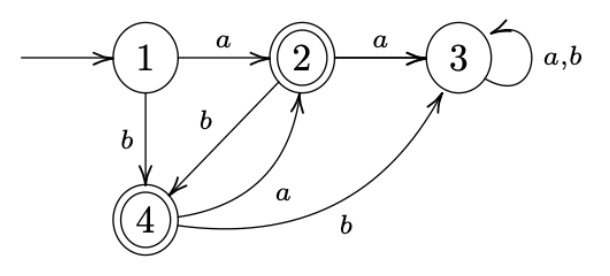
\includegraphics[width=0.45\textwidth]{A1hw2.png}}{\fbox{\parbox{0.4\textwidth}{\centering [Insert $\mathcal{A}^{(1)}$]}}}\quad
  \IfFileExists{A2hw2.png}{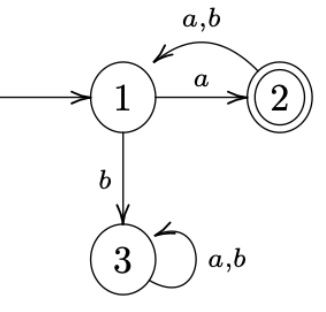
\includegraphics[width=0.45\textwidth]{A2hw2.png}}{\fbox{\parbox{0.4\textwidth}{\centering [Insert $\mathcal{A}^{(2)}$]}}}
  \caption{$\mathcal{A}^{(1)}$ (left) and $\mathcal{A}^{(2)}$ (right).}
  \label{fig:A12}
\end{figure}

\begin{enumerate}
  \item \textbf{Describe $L(\mathcal{A}^{(1)})$ and $L(\mathcal{A}^{(2)})$.}
  
  \textbf{Answer:}
  \begin{itemize}
    \item $L(\mathcal{A}^{(1)})$: Words include $a$, $b$, $ba$, $bab$, $baba$, $ab$, $aba$, $abab$, etc. I can see that each character must alternate based on its successive character.
    \item $L(\mathcal{A}^{(2)})$: Words include $a$, $axa$ (where $x$ doesn't matter). I see the word must start with $a$, and must add to its word length in increments of 2, every other character being $a$.
  \end{itemize}
  
  \item \textbf{Construct the intersection automaton $\mathcal{A}$ for $\mathcal{A}^{(1)}$ and $\mathcal{A}^{(2)}$ by drawing its transition diagram (omit unreachable states).}
  
  \textbf{Answer:}
  Below is the intersection automaton diagram.
  \begin{figure}[H]
    \centering
    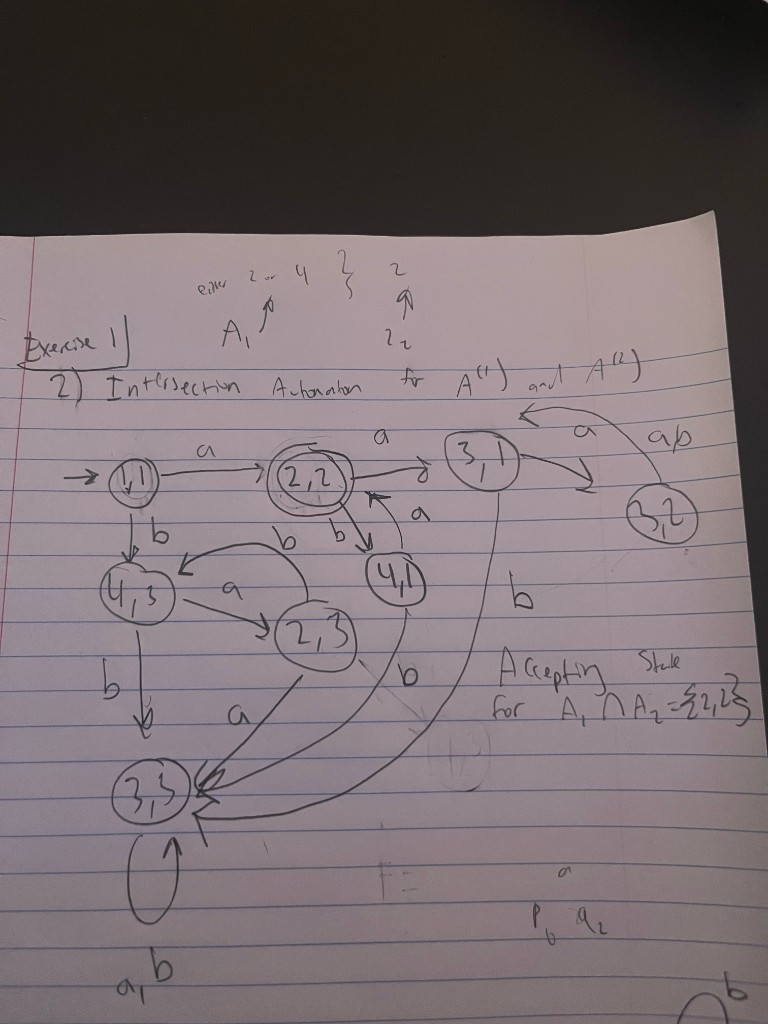
\includegraphics[width=0.85\textwidth]{ex1-intersection.png}
    \caption{Intersection automaton $\mathcal{A}$ for $\mathcal{A}^{(1)}$ and $\mathcal{A}^{(2)}$ (omit unreachable states).}
    \label{fig:ex1q2dfa}
  \end{figure}
  \noindent\textit{Note:} $\{2,2\}$ as accepting state for intersection product automaton.
  
  \item \textbf{Argue that $L(\mathcal{A}) = L(\mathcal{A}^{(1)}) \cap L(\mathcal{A}^{(2)})$.}
  
  \textbf{Answer:}
  Since $L(\mathcal{A}^{(1)})$ includes words such as $a$, $b$, $ba$, $bab$, $baba$ and $ab$, $aba$, $abab$, and $L(\mathcal{A}^{(2)})$ includes words that (1) must start with $a$---so we can disregard the words that start with $b$ in $L(\mathcal{A}^{(1)})$, leaving us with $a$, $ab$, $aba$, etc.---and (2) the requirement for $L(\mathcal{A}^{(2)})$ is to be in increments of two, we are left with patterns: $a$, $aba$, $ababa$, etc. Thus we obtain the automaton of both intersection.
  
  \item \textbf{How can you change $\mathcal{A}$ to get an automaton $\mathcal{A}'$ with $L(\mathcal{A}') = L(\mathcal{A}^{(1)}) \cup L(\mathcal{A}^{(2)})$?}
  
  \textbf{Answer:}
  In the product automaton we would add the accepting states to not be exclusive to both, but inclusive of either one of the subset DFA's accepting state.
\end{enumerate}

\subsubsection*{Exercise 2 (More automata)}

Consider the following automata $\mathcal{B}^{(1)}$ and $\mathcal{B}^{(2)}$.

\begin{figure}[ht]
  \centering
  \IfFileExists{B1hw2.png}{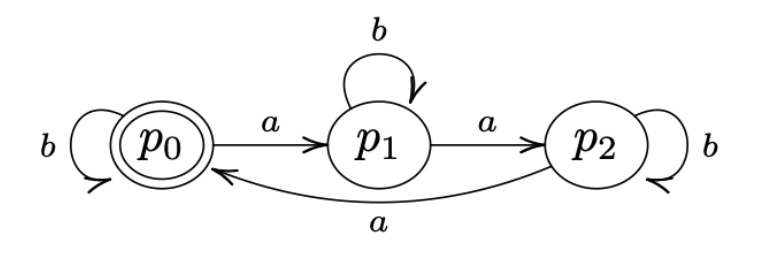
\includegraphics[width=0.45\textwidth]{B1hw2.png}}{\fbox{\parbox{0.4\textwidth}{\centering [Insert $\mathcal{B}^{(1)}$]}}}\quad
  \IfFileExists{B2hw2.png}{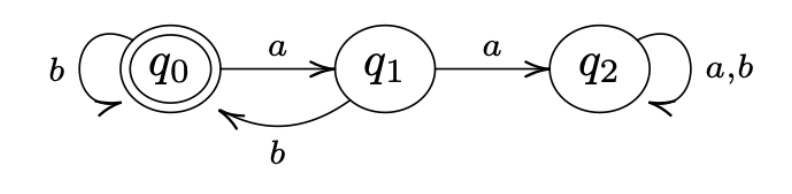
\includegraphics[width=0.45\textwidth]{B2hw2.png}}{\fbox{\parbox{0.4\textwidth}{\centering [Insert $\mathcal{B}^{(2)}$]}}}
  \caption{$\mathcal{B}^{(1)}$ (left) and $\mathcal{B}^{(2)}$ (right).}
  \label{fig:B12}
\end{figure}

(Recall: the complement of a language $L \subseteq \Sigma^*$ is $\overline{L} := \Sigma^* \setminus L$.)



\begin{enumerate}
  \item \textbf{Describe $L(\mathcal{B}^{(1)})$ and $L(\mathcal{B}^{(2)})$.}
  
  \textbf{Answer:}
  \begin{figure}[H]
    \centering
    \caption{$L(\mathcal{B}^{(1)})$ rules: include 3 $a$'s at a time, any amount of $b$'s. $L(\mathcal{B}^{(2)})$ rules: $b$ must follow an $a$, any amount of $b$'s. DFA diagram for language 2.}
    \label{fig:ex2notes}
  \end{figure}
  
  \item \textbf{Construct the intersection automaton $\mathcal{B}$ for $\mathcal{B}^{(1)}$ and $\mathcal{B}^{(2)}$ (omit unreachable states).}
  
  \textbf{Answer:}
  Below is the intersection automaton diagram.
  \begin{figure}[H]
    \centering
    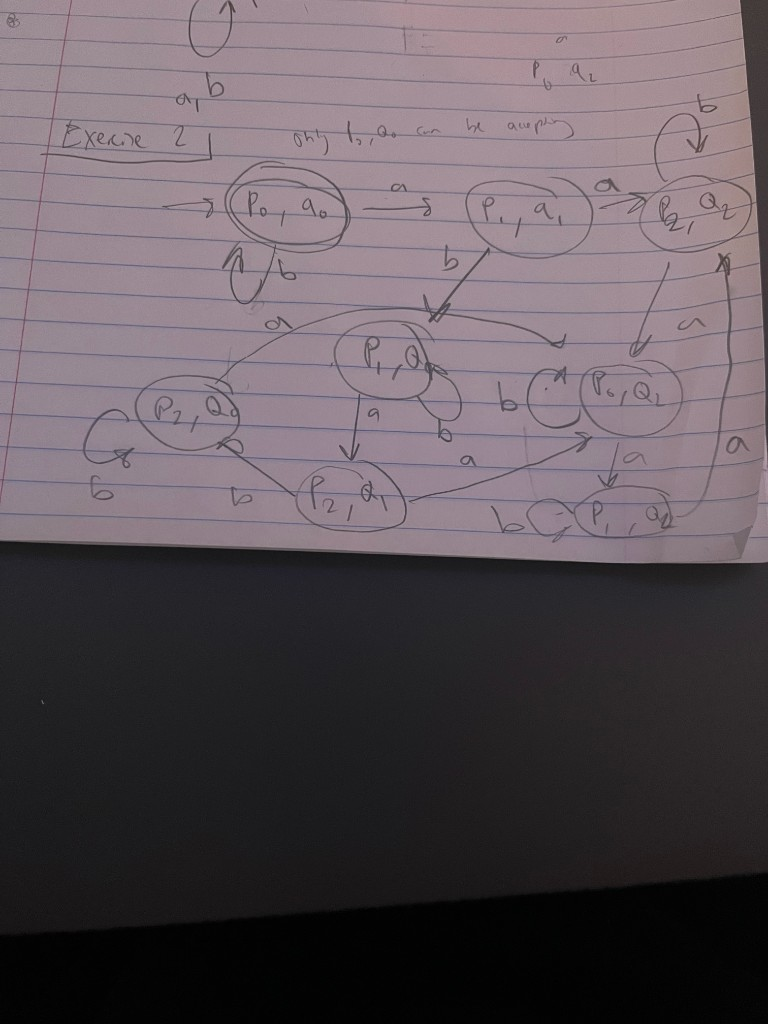
\includegraphics[width=0.85\textwidth]{ex2-intersection.png}
    \caption{Intersection automaton $\mathcal{B}$ for $\mathcal{B}^{(1)}$ and $\mathcal{B}^{(2)}$ (omit unreachable states).}
    \label{fig:ex2intersection}
  \end{figure}
  \noindent\textit{Note:} $(P_0, Q_0)$ as accepting state.
  
  \item \textbf{Argue that $L(\mathcal{B}) = L(\mathcal{B}^{(1)}) \cap L(\mathcal{B}^{(2)})$.}
  
  \textbf{Answer:}
  Both automata have the rule that any amount of $b$'s is allowed. But we must combine the rules regarding $a$'s. $L(\mathcal{B}^{(1)})$ requires 3 $a$'s to be included at a time per word, while $\mathcal{B}^{(2)}$ requires the rule that $a$ must be followed by a $b$. This gives us the conclusion that words that do include an $a$ must come in pairs of 3 $a$'s with $b$ following the last $a$.
  
  \item \textbf{How can you change $\mathcal{B}$ to get an automaton $\mathcal{B}'$ with $L(\mathcal{B}') = L(\mathcal{B}^{(1)}) \cup \overline{L(\mathcal{B}^{(2)})}$?}
  
  \textbf{Answer:}
  The Union is equivalent to its intersection, no possible change.
\end{enumerate}

\subsubsection*{Exercise 3}
Let $\mathcal{A}$ be a DFA and $q$ a state of $\mathcal{A}$ such that from $q$, every input symbol $a$ leaves us in $q$ (i.e.\ $\delta(q,a) = q$ for all $a$). Show by induction on the length of the input that for any input string $w$, we still end up in $q$ (i.e.\ $\delta^*(q,w) = q$).

\textbf{Answer:}
We show it by induction on the length of $w$. (Here $\delta^*(q,w)$ is just the state we end up in after starting at $q$ and reading the whole string $w$.)

When the input has length $0$, the string is empty. So we don't read anything and we stay at $q$. So $\delta^*(q,w) = q$ in that case.

Now suppose we've already shown that for every string of length $n$, we end up back at $q$. Take a string $w$ of length $n+1$. We can write it as $w = va$ (some string $v$ of length $n$ plus one symbol $a$). After reading $v$ we're in $\delta^*(q,v)$, and by our assumption that's $q$. Then we read $a$, and we're in $\delta(q,a)$, which is $q$ by the given rule. So after reading $w$ we're still in $q$, i.e.\ $\delta^*(q,w) = q$.

So by induction, for all input strings $w$ we have $\delta^*(q,w) = q$.

\subsubsection*{Question}
If you build the product automaton for $\mathcal{B}^{(1)}$ and $\mathcal{B}^{(2)}$ but change the accepting set to get the \emph{union} $L(\mathcal{B}^{(1)}) \cup L(\mathcal{B}^{(2)})$ instead of the intersection, how many states must be accepting?

\subsection{Week 3}\label{sec:week3}

\subsubsection*{Homework 1 (NFA)}
\begin{enumerate}
  \item Describe the language accepted by $\mathcal{A}$ using a regular expression.
  \item Specify the NFA $\mathcal{A}$ in the form $(Q, \Sigma, \delta, q_0, F)$.
  \item Find all paths in $\mathcal{A}$ for the word $w = abab$; represent in a diagram.
  \item Construct the determinization $\mathcal{A}^D$ of $\mathcal{A}$ using the power set construction. Create both a transition table and a graphical depiction of $\mathcal{A}^D$.
\end{enumerate}

\paragraph{Answer (NFA specification).}
Here is how I write the NFA $\mathcal{A}$ formally:
\[
Q = \{0,1,2,3\}, \qquad
\Sigma = \{a,b,c\}, \qquad
q_0 = 0, \qquad
F = \{2,3\}.
\]
For the transition function $\delta : Q \times \Sigma \to \mathcal{P}(Q)$ I use
\[
\begin{aligned}
  \delta(0,a) &= \{0,1\}, &
  \delta(0,b) &= \{0\}, &
  \delta(0,c) &= \emptyset, \\
  \delta(1,b) &= \{2\}, &
  \delta(1,c) &= \{2\},
\end{aligned}
\]
and any transition not listed goes to the empty set (i.e.\ there is no move).

\begin{figure}[H]
  \centering
  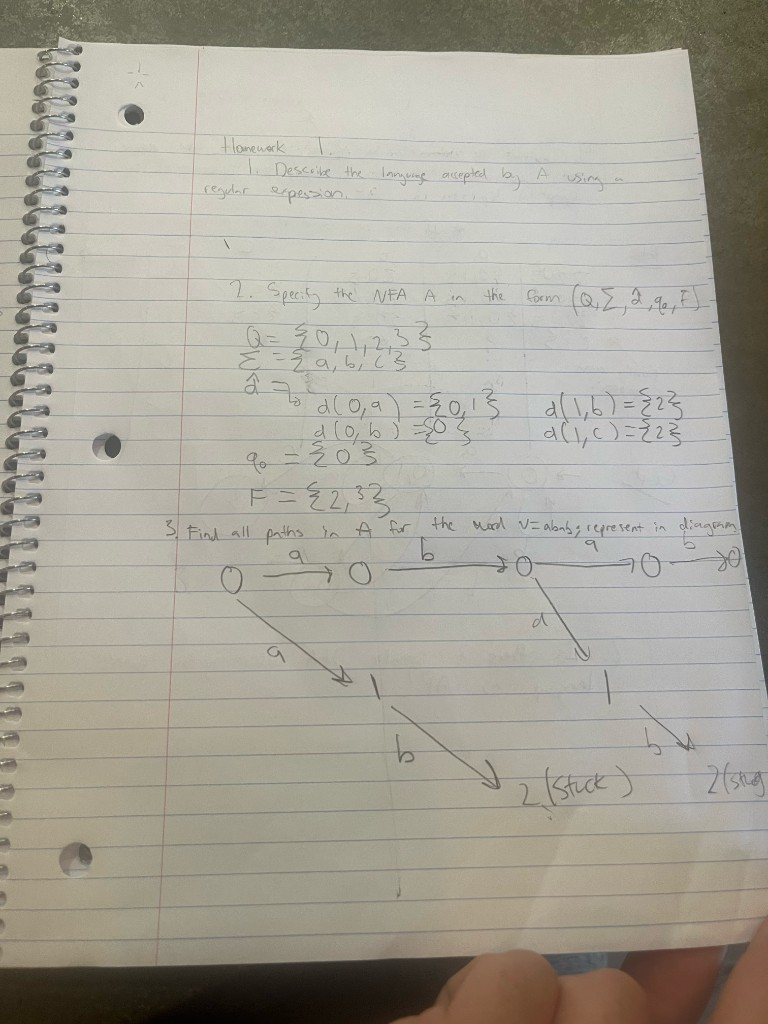
\includegraphics[width=0.9\textwidth]{week3-hw1.png}
  \caption{Homework 1: NFA specification $(Q=\{0,1,2,3\}$, $\Sigma=\{a,b,c\}$, $q_0=0$, $F=\{2,3\})$ and all paths for $w=abab$.}
  \label{fig:week3hw1}
\end{figure}

\paragraph{Transition table for $\mathcal{A}^D$ over $\{a,b,c\}$.}
From my construction I focus on the following subset-states:
\[
\{0\},\ \{0,1\},\ \{0,2\},\ \{3\}.
\]
The transitions on $a$, $b$, and $c$ are:

\begin{center}
\begin{tabular}{|c|c|c|c|}
  \hline
  State $S$ & on input $a$ & on input $b$ & on input $c$ \\
  \hline
  $\{0\}$   & $\{0,1\}$ & $\{0\}$   & $\emptyset$ \\
  $\{0,1\}$ & $\{0,1\}$ & $\{0,2\}$ & $\{3\}$     \\
  $\{0,2\}$ & $\{0,1\}$ & $\{0\}$   & $\emptyset$ \\
  $\{3\}$   & $\emptyset$ & $\emptyset$ & $\emptyset$ \\
  \hline
\end{tabular}
\end{center}

\begin{figure}[H]
  \centering
  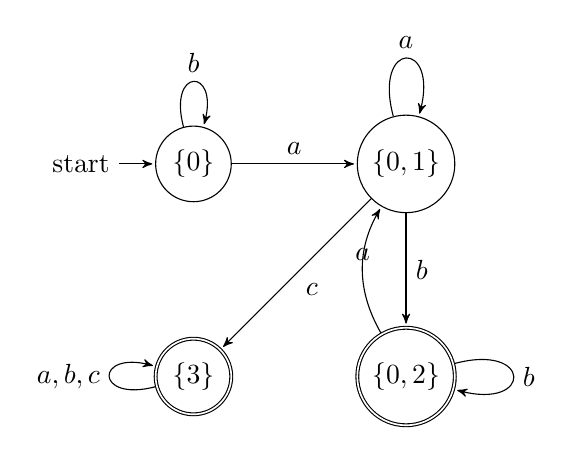
\begin{tikzpicture}[>=stealth',shorten >=1pt,node distance=2.7cm,on grid,auto]
    \node[state,initial] (s0) {$\{0\}$};
    \node[state] (s01) [right=of s0] {$\{0,1\}$};
    \node[state,accepting] (s02) [below=of s01] {$\{0,2\}$};
    \node[state,accepting] (s3) [below=of s0] {$\{3\}$};

    \path[->]
      (s0)  edge[loop above] node {$b$} ()
            edge node {$a$} (s01)
      (s01) edge[loop above] node {$a$} ()
            edge node[right] {$b$} (s02)
            edge node {$c$} (s3)
      (s02) edge[loop right] node {$b$} ()
            edge[bend left] node[above] {$a$} (s01)
      (s3)  edge[loop left] node {$a,b,c$} ();
  \end{tikzpicture}
  \caption{Determinized DFA $\mathcal{A}^D$ for Homework 2 over alphabet $\{a,b,c\}$. Accepting states are the subsets that contain an original accepting state ($\{0,2\}$ and $\{3\}$).}
  \label{fig:week3hw2}
\end{figure}

\subsubsection*{Homework 2 (DFA and minimization)}
Determine $\mathcal{A}^D$ of $\mathcal{A}$ using the power set construction, now with alphabet $\{0,1\}$. Create both a transition table and a graphical depiction of $\mathcal{A}^D$. Then decide whether there can be a smaller DFA accepting the same language.

\paragraph{Transition table over $\{0,1\}$.}
From the NFA given in the homework, I use the following subset-states:
\[
q_0,\ \{q_0,q_1\},\ \{q_0,q_1,q_2\},\ \{q_0,q_3\},\ \{q_0,q_1,q_3\},\ \{q_0,q_1,q_2,q_3\}.
\]
The determinized DFA $\mathcal{A}^D$ then has this transition table:

\begin{center}
\begin{tabular}{|c|c|c|}
  \hline
  State $S$ & on input $0$ & on input $1$ \\
  \hline
  $q_0$                     & $q_0$                   & $\{q_0,q_1\}$ \\
  $\{q_0,q_1\}$             & $q_0$                   & $\{q_0,q_1,q_2\}$ \\
  $\{q_0,q_1,q_2\}$         & $\{q_0,q_3\}$           & $\{q_0,q_1,q_2\}$ \\
  $\{q_0,q_3\}$             & $\{q_0,q_3\}$           & $\{q_0,q_1,q_3\}$ \\
  $\{q_0,q_1,q_3\}$         & $\{q_0,q_3\}$           & $\{q_0,q_1,q_2,q_3\}$ \\
  $\{q_0,q_1,q_2,q_3\}$     & $\{q_0,q_3\}$           & $\{q_0,q_1,q_2,q_3\}$ \\
  \hline
\end{tabular}
\end{center}

Any subset that contains the original accepting state(s) is accepting in $\mathcal{A}^D$.

\paragraph{Smaller DFA?}
Yes. In this table the last two rows (for $\{q_0,q_1,q_2,q_3\}$ and for $\{q_0,q_3\}$) have exactly the same outgoing transitions and the same accepting/non-accepting status. That means these two states are equivalent and can be merged into a single state, giving a smaller DFA that still recognizes the same language.

\begin{figure}[H]
  \centering
  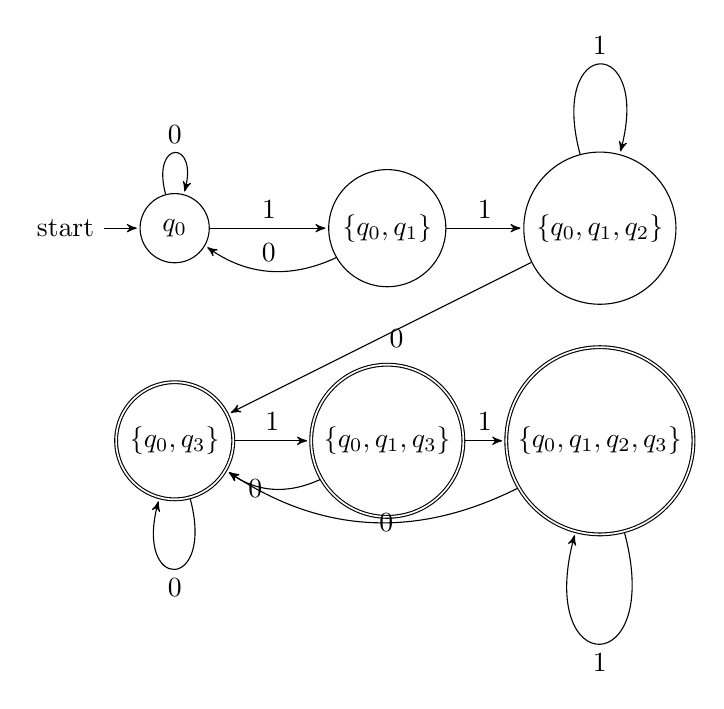
\begin{tikzpicture}[>=stealth',shorten >=1pt,node distance=2.7cm,on grid,auto]
    \node[state,initial] (q0) {$q_0$};
    \node[state] (q01) [right=of q0] {$\{q_0,q_1\}$};
    \node[state] (q012) [right=of q01] {$\{q_0,q_1,q_2\}$};
    \node[state,accepting] (q03) [below=of q0] {$\{q_0,q_3\}$};
    \node[state,accepting] (q013) [below=of q01] {$\{q_0,q_1,q_3\}$};
    \node[state,accepting] (q0123) [below=of q012] {$\{q_0,q_1,q_2,q_3\}$};

    \path[->]
      (q0) edge[loop above] node {$0$} ()
           edge node {$1$} (q01)
      (q01) edge[bend left] node[above] {$0$} (q0)
            edge node {$1$} (q012)
      (q012) edge node[right] {$0$} (q03)
             edge[loop above] node {$1$} ()
      (q03) edge[loop below] node {$0$} ()
            edge node {$1$} (q013)
      (q013) edge[bend left] node[left] {$0$} (q03)
             edge node {$1$} (q0123)
      (q0123) edge[bend left] node[right] {$0$} (q03)
              edge[loop below] node {$1$} ();
  \end{tikzpicture}
  \caption{Determinized DFA $\mathcal{A}^D$ for Homework 2 over alphabet $\{0,1\}$. Accepting states are the subsets that contain the original accepting state $q_3$.}
  \label{fig:week3hw3}
\end{figure}

\subsubsection*{Question}
After building $\mathcal{A}^D$ from an NFA $\mathcal{A}$ using the power set construction, when can we get a smaller DFA that still accepts the same language? 

\subsection{Week 4}\label{sec:week4}

Consider the following DFA $\mathcal{A}$: there is a state $p$ (initial and final) with transition $a$ to itself and transition $b$ to state $q$; state $q$ has transition $b$ to itself and transition $a$ to $p$.

\begin{figure}[H]
  \centering
  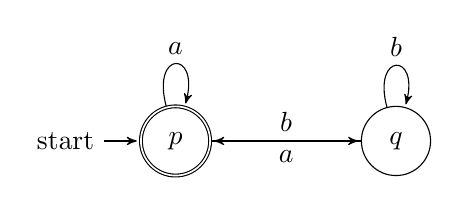
\begin{tikzpicture}[>=stealth',shorten >=1pt,node distance=2.8cm,on grid,auto]
    \node[state,initial,accepting] (p) {$p$};
    \node[state] (q) [right=of p] {$q$};
    \path[->]
      (p) edge[loop above] node {$a$} ()
          edge node[above] {$b$} (q)
      (q) edge[loop above] node {$b$} ()
          edge node[below] {$a$} (p);
  \end{tikzpicture}
  \caption{DFA $\mathcal{A}$ for Week 4: $p$ is initial and final; $p \xrightarrow{a} p$, $p \xrightarrow{b} q$, $q \xrightarrow{b} q$, $q \xrightarrow{a} p$.}
  \label{fig:week4dfa}
\end{figure}

\paragraph{Question.} For $p = 1$ and $q = 2$, compute via Kleene's algorithm all regular expressions $R^{(k)}_{ij}$ and from this a resulting regular expression $R$ describing $L(\mathcal{A})$, i.e., such that $L(R) = L(\mathcal{A})$.

\paragraph{Answer.} I label the states so that state $1$ is $p$ and state $2$ is $q$. In Kleene's algorithm, $R^{(k)}_{ij}$ denotes the set of all strings that label paths from $i$ to $j$ with intermediate states (if any) in $\{1,\ldots,k\}$. The recurrence is
\[
R^{(k)}_{ij} = R^{(k-1)}_{ij} \cup R^{(k-1)}_{ik} \bigl(R^{(k-1)}_{kk}\bigr)^* R^{(k-1)}_{kj}.
\]
I write union as $+$ in expressions below.

\paragraph{Base case $k=0$} (no intermediate states; only direct edges and $\varepsilon$ on same state):
\[
R^{(0)}_{11} = \varepsilon + a,\qquad
R^{(0)}_{12} = b,\qquad
R^{(0)}_{21} = a,\qquad
R^{(0)}_{22} = \varepsilon + b.
\]

\paragraph{Inductive step $k=1$} (intermediate state 1 allowed). Using $(R^{(0)}_{11})^* = (\varepsilon+a)^* = a^*$:
\begin{align*}
R^{(1)}_{11} &= R^{(0)}_{11} + R^{(0)}_{11}(R^{(0)}_{11})^* R^{(0)}_{11} = (\varepsilon+a) + (\varepsilon+a)a^*(\varepsilon+a) = a^*; \\
R^{(1)}_{12} &= R^{(0)}_{12} + R^{(0)}_{11}(R^{(0)}_{11})^* R^{(0)}_{12} = b + (\varepsilon+a)a^* b = a^*b; \\
R^{(1)}_{21} &= R^{(0)}_{21} + R^{(0)}_{21}(R^{(0)}_{11})^* R^{(0)}_{11} = a + a\,a^*(\varepsilon+a) = a\,a^*; \\
R^{(1)}_{22} &= R^{(0)}_{22} + R^{(0)}_{21}(R^{(0)}_{11})^* R^{(0)}_{12} = (\varepsilon+b) + a\,a^* b = (\varepsilon+b) + a^+b.
\end{align*}

\paragraph{Inductive step $k=2$} (all states allowed). Set $C = R^{(1)}_{22} = (\varepsilon+b) + a^+b = b + a^+b$ (since $\varepsilon+b$ gives $\varepsilon$ and $b$). Then $(R^{(1)}_{22})^* = (b + a^+b)^*$. Only state $1$ is accepting, so $L(\mathcal{A})$ is the set of strings that label paths from $1$ to $1$:
\[
R^{(2)}_{11} = R^{(1)}_{11} + R^{(1)}_{12}\,\bigl(R^{(1)}_{22}\bigr)^* R^{(1)}_{21}
= a^* + a^*b\,(b+a^+b)^*\,a^+.
\]
Thus a regular expression $R$ with $L(R) = L(\mathcal{A})$ is
\[
\boxed{R \;=\; a^* + a^*b\,(b+a^+b)^*\,a^+}.
\]
(Here $a^+ = aa^*$; one can also write $a^*b\,(b \cup a^+b)^*\,a^+$ if union is denoted $\cup$.)

\subsubsection*{Question}
If we changed the DFA so that both $p$ and $q$ were accepting states, how would the regular expression $R$ for $L(\mathcal{A})$ change? Would it simplify to a shorter expression?

\subsection{Week 5}\label{sec:week5}

\subsubsection*{Exercise (Pumping lemma and non-regular languages)}
Show that the following languages are not regular using the pumping lemma:
\[
L_1 = \{ a^n b^m \in \{a,b\}^* \mid n,m \in \mathbb{N},\ n > m \ge 0 \},
\]
\[
L_2 = \{ a^{n^2} \in \{a\}^* \mid n \in \mathbb{N},\ n \ge 1 \},
\]
\[
L_3 = \{ a^p \in \{a\}^* \mid p \in \mathbb{N},\ p \text{ prime} \},
\]
\[
L_4 = \{ a^k b^m a^{k+m} \mid k,m \ge 0 \}.
\]

\paragraph{1. Showing $L_1$ is not regular.}
I assume $L_1$ is regular and take a pumping constant $p$ from the lemma. I pick the string
\[
w = a^{p+1} b^{p} \in L_1,
\]
since here $n = p+1$ and $m = p$ so indeed $n > m$. By the pumping lemma I can write $w = xyz$ with $|xy| \le p$, $|y| \ge 1$, and for all $i \ge 0$ the pumped string $xy^i z$ should still be in $L_1$.\newline
Because $|xy| \le p$ and $w$ starts with only $a$'s, the substring $y$ must consist entirely of $a$'s. So say $y = a^t$ with $t \ge 1$. If I pump down with $i = 0$, I get the string
\[
xy^0 z = xz = a^{p+1 - t} b^p,
\]
so the number of $a$'s in this string is $p+1-t$, and the number of $b$'s is still $p$. Since $t \ge 1$, I now have $p+1-t \le p$, so $n \le m$ for this pumped string. That means $xy^0 z \notin L_1$, contradicting the pumping lemma. So my assumption that $L_1$ was regular must be wrong; $L_1$ is not regular.

\paragraph{2. Showing $L_2$ is not regular.}
Again I assume $L_2$ is regular and let $p$ be the pumping length. I choose
\[
w = a^{p^2} \in L_2,
\]
since $p^2$ is a perfect square. The lemma gives me a split $w = xyz$ with $|xy| \le p$, $|y| \ge 1$, and $xy^i z \in L_2$ for all $i \ge 0$. Because the whole word is just $a$'s and $|xy| \le p$, I know that $y = a^t$ for some $1 \le t \le p$.\newline
Now I pump once with $i = 2$. Then
\[
xy^2 z = a^{p^2 + t}.
\]
If this were in $L_2$, I would need $p^2 + t = n^2$ for some integer $n$. But $1 \le t \le p$, so $p^2 < p^2 + t < (p+1)^2 = p^2 + 2p + 1$. There is no perfect square strictly between $p^2$ and $(p+1)^2$, so $p^2 + t$ cannot be a square. Hence $xy^2 z \notin L_2$, contradicting the pumping lemma. So $L_2$ is not regular.

\paragraph{3. Showing $L_3$ is not regular.}
I assume $L_3$ is regular and take its pumping length $p$. Choose $w = a^q \in L_3$ where $q$ is any prime number with $q \ge p$ (there are infinitely many primes, so I can definitely pick one large enough). Then $w = xyz$ with $|xy| \le p$, $|y| \ge 1$, and $xy^i z \in L_3$ for all $i \ge 0$. As before, $y = a^t$ where $1 \le t \le p$.\newline
The length of $w$ is $q$, and the length of $xy^i z$ is $q + (i-1)t$. I look at $i = q+1$ to pump a bunch of copies of $y$:
\[
|xy^{q+1} z| = q + q t = q(1+t).
\]
This number is clearly a composite (product of $q$ and $1+t$, both $>1$), so it is not prime. That means $xy^{q+1} z \notin L_3$, contradicting the pumping lemma. Therefore $L_3$ is not regular.

\paragraph{4. Showing $L_4$ is not regular.}
Assume $L_4$ is regular and let $p$ be its pumping length. I pick
\[
w = a^{p} b^{p} a^{2p} \in L_4,
\]
since here $k = p$ and $m = p$, so the last block is $a^{k+m} = a^{2p}$. The pumping lemma says $w = xyz$ with $|xy| \le p$, $|y| \ge 1$, and $xy^i z \in L_4$ for all $i \ge 0$. Because $|xy| \le p$ and the first $p$ symbols are $a$'s, the piece $y$ sits entirely in the first block of $a$'s. So $y = a^t$ for some $1 \le t \le p$.\newline
If I pump with $i = 2$, the new word is
\[
xy^2 z = a^{p+t} b^{p} a^{2p}.
\]
In this string, the leftmost block of $a$'s has length $k' = p+t$, the $b$-block has length $m' = p$, but the rightmost block is still $a^{2p}$, i.e.\ length $2p$. For this to be in $L_4$ I would need the last block to have length $k' + m' = (p+t) + p = 2p + t$. That would mean I need $2p = 2p + t$, which is impossible since $t \ge 1$. So $xy^2z \notin L_4$, contradicting the pumping lemma. Hence $L_4$ is not regular.

\subsubsection*{Question}
In these pumping-lemma proofs I always picked one very specific string $w$ in each language. How much freedom do I actually have in choosing $w$? Could I have picked a different family of strings (for example, $a^{p+2}b^{p+1}$ for $L_1$) and still made the same argument work just as well?

\subsection{Week 6}\label{sec:week6}

\subsubsection*{Exercise A (Turing machines)}
Write a TM to accept the language of binary strings
\[
L = \{ 1 0^n \mid n \in \mathbb{N} \}
\]
and for the input $10^n$ it returns the string $10^{n+1}$. Write a TM to accept the same language $L$ and for input $10^n$ it returns the string $1$. Write a TM to accept the total language of binary strings and, for every string, it returns the string with $0$'s and $1$'s swapped.

\paragraph{Conventions.}
My tape alphabet is $\Gamma = \{0,1,\blank\}$ and the head starts on the leftmost symbol of the input. When I say the machine ``returns'' an output string, I mean it halts with the output written on the tape (starting at the leftmost cell).

\paragraph{1) TM for $L=\{10^n\}$ that outputs $10^{n+1}$.}
Idea: verify the input is $1$ followed by only $0$'s; scan to the first blank and write one more $0$.

\[
M_1 = (Q,\Sigma,\Gamma,\delta,q_s,q_{acc},q_{rej})
\]
where $\Sigma=\{0,1\}$, $\Gamma=\{0,1,\blank\}$, and the states are
\[
Q=\{q_s,q_{z},q_{acc},q_{rej}\}.
\]
The transition function $\delta$ is:

\begin{center}
\begin{tabular}{|c|c|c|}
  \hline
  state / read & write, move & next state \\
  \hline
  $q_s$ on $1$ & write $1$, $R$ & $q_z$ \\
  $q_s$ on $0$ & write $0$, $R$ & $q_{rej}$ \\
  $q_s$ on $\blank$ & write $\blank$, $R$ & $q_{rej}$ \\
  \hline
  $q_z$ on $0$ & write $0$, $R$ & $q_z$ \\
  $q_z$ on $1$ & write $1$, $R$ & $q_{rej}$ \\
  $q_z$ on $\blank$ & write $0$, $S$ & $q_{acc}$ \\
  \hline
\end{tabular}
\end{center}

So if the input is $10^n$, it halts with $10^{n+1}$ on the tape. If the input is not in $L$, it rejects.

\paragraph{2) TM for $L=\{10^n\}$ that outputs $1$.}
Idea: verify the same language, then erase everything to the right of the first $1$.

\[
M_2 = (Q,\Sigma,\Gamma,\delta,q_s,q_{acc},q_{rej})
\]
with $\Sigma=\{0,1\}$, $\Gamma=\{0,1,\blank\}$, and
\[
Q=\{q_s,q_{z},q_{back},q_{clr},q_{acc},q_{rej}\}.
\]
Transitions:

\begin{center}
\begin{tabular}{|c|c|c|}
  \hline
  state / read & write, move & next state \\
  \hline
  $q_s$ on $1$ & write $1$, $R$ & $q_z$ \\
  $q_s$ on $0$ & write $0$, $R$ & $q_{rej}$ \\
  $q_s$ on $\blank$ & write $\blank$, $R$ & $q_{rej}$ \\
  \hline
  $q_z$ on $0$ & write $0$, $R$ & $q_z$ \\
  $q_z$ on $1$ & write $1$, $R$ & $q_{rej}$ \\
  $q_z$ on $\blank$ & write $\blank$, $L$ & $q_{back}$ \\
  \hline
  $q_{back}$ on $0$ & write $0$, $L$ & $q_{back}$ \\
  $q_{back}$ on $1$ & write $1$, $R$ & $q_{clr}$ \\
  \hline
  $q_{clr}$ on $0$ & write $\blank$, $R$ & $q_{clr}$ \\
  $q_{clr}$ on $\blank$ & write $\blank$, $S$ & $q_{acc}$ \\
  \hline
\end{tabular}
\end{center}

When it accepts, the only nonblank symbol left from the original input is the first $1$, so the tape contains output $1$.

\paragraph{3) TM on all binary strings that swaps $0$ and $1$.}
Idea: sweep left-to-right and flip each bit; accept when we hit blank.

\[
M_3 = (Q,\Sigma,\Gamma,\delta,q_s,q_{acc})
\]
where $\Sigma=\{0,1\}$, $\Gamma=\{0,1,\blank\}$,
\[
Q=\{q_s,q_{acc}\},
\]
and $\delta$ is:

\begin{center}
\begin{tabular}{|c|c|c|}
  \hline
  state / read & write, move & next state \\
  \hline
  $q_s$ on $0$ & write $1$, $R$ & $q_s$ \\
  $q_s$ on $1$ & write $0$, $R$ & $q_s$ \\
  $q_s$ on $\blank$ & write $\blank$, $S$ & $q_{acc}$ \\
  \hline
\end{tabular}
\end{center}

This accepts every binary string and halts with all bits flipped.

\subsubsection*{Exercise 1 (Decidable vs.\ r.e.\ closure properties)}
Which of the following statements is true? If yes, give an argument; if no, give a counterexample.

\begin{enumerate}
  \item \textbf{If $L_1$ and $L_2$ are decidable, then so is $L_1 \cup L_2$.}
  
  \textbf{True.} If $D_1$ decides $L_1$ and $D_2$ decides $L_2$, then a decider for $L_1 \cup L_2$ is: on input $w$, run $D_1(w)$ and $D_2(w)$. Accept iff at least one of them accepts. Since both halt on every input, this procedure halts on every input too.
  
  \item \textbf{If $L$ is decidable, then so is the complement $\overline{L} := \Sigma^* \setminus L$.}
  
  \textbf{True.} If $D$ decides $L$, then a decider for $\overline{L}$ is: on input $w$, run $D(w)$ and flip the answer (accept $\leftrightarrow$ reject). It still halts on every input.
  
  \item \textbf{If $L$ is decidable, then so is $L^*$.}
  
  \textbf{True.} Let $D$ be a decider for $L$. Given a word $w$ of length $n$, there are only finitely many ways to split $w$ into a concatenation $w = x_1 x_2 \cdots x_t$ (with $t \ge 0$ and each $x_i \in \Sigma^*$; allowing $t=0$ gives $\varepsilon$). I can decide whether $w \in L^*$ by checking all splits and accepting iff there exists a split where $D(x_i)$ accepts for every piece $x_i$. This always halts because there are finitely many splits and $D$ always halts.
  
  \item \textbf{If $L_1$ and $L_2$ are r.e., then $L_1 \cup L_2$ is r.e.}
  
  \textbf{True.} Let $R_1$ and $R_2$ be recognizers for $L_1$ and $L_2$. A recognizer for $L_1 \cup L_2$ can dovetail them: on input $w$, simulate $R_1(w)$ and $R_2(w)$ in parallel (one step of each, alternating). If either one accepts, accept. If $w \in L_1 \cup L_2$, at least one recognizer will accept in finite time, so this machine accepts in finite time.
  
  \item \textbf{If $L$ is r.e., then so is $\overline{L}$.}
  
  \textbf{False.} A standard counterexample is the acceptance problem
  \[
  A_{TM} = \{ \langle M,w\rangle \mid M \text{ accepts } w\}.
  \]
  We know $A_{TM}$ is r.e.\ (simulate $M$ on $w$ and accept if it accepts), but $\overline{A_{TM}}$ is \emph{not} r.e. (if both were r.e., then $A_{TM}$ would be decidable by running the two recognizers in parallel and waiting for one to accept, which is impossible).
  
  \item \textbf{If $L$ is r.e., then so is $L^*$.}
  
  \textbf{True.} Let $R$ be a recognizer for $L$. To recognize $L^*$ on input $w$, I can enumerate all splits of $w$ into pieces $w = x_1 \cdots x_t$ and dovetail all the computations that check ``$x_1 \in L$ and $\cdots$ and $x_t \in L$'' (each check is a finite list of runs of $R$). If for some split every piece is accepted by $R$, then accept $w$. If $w \in L^*$, there exists such a split, and all those runs accept in finite time, so this procedure will eventually accept.
\end{enumerate}

\subsubsection*{Question}
When I argue something is decidable vs.\ only r.e., what is the key difference in the machine behavior I'm relying on? Is it basically always ``will it halt on the reject cases''?

\subsection{Week 7}\label{sec:week7}

\subsubsection*{Exercise 2 (Decidability)}
Argue for each of the languages $L_1$, $L_2$, $L_3$ whether they are decidable, recursively enumerable (r.e.), or have recursively enumerable complement (co-r.e.).
\begin{align*}
L_1 &:= \{ M \mid \text{$M$ halts on itself} \}, \\
L_2 &:= \{ (M,w) \mid \text{$M$ halts on the word $w$} \}, \\
L_3 &:= \{ (M,w,k) \mid \text{$M$ halts on $w$ in at most $k$ steps} \}.
\end{align*}

\paragraph{Answer.}
I treat inputs as valid encodings of Turing machines (and tuples) over a fixed alphabet.

\paragraph{$L_2$ (the halting problem).}
$L_2$ is \textbf{not decidable} (Turing's theorem). It \textbf{is r.e.}: on input $(M,w)$, simulate $M$ on $w$ step by step; if $M$ ever halts, accept. If $(M,w)$ is a yes-instance, this simulation eventually halts and we accept. If $M$ never halts on $w$, the simulator runs forever, so we never reject---which is fine for recognition.

The complement $\overline{L_2}$ is \textbf{not r.e.}: if both $L_2$ and $\overline{L_2}$ were r.e., we could run recognizers in parallel and decide halting, contradicting undecidability. So $L_2$ is r.e.\ but not co-r.e.

\paragraph{$L_1$.}
$L_1$ is essentially the same phenomenon as halting, with a fixed input (the encoding of $M$ itself). It is \textbf{not decidable}: if we had a decider for $L_1$, we could decide $L_2$ as follows---given $(M,w)$, build a machine $M_w$ that ignores its input and simulates $M$ on $w$; then $M_w$ halts on every input (in particular on itself) iff $M$ halts on $w$. So decidability of $L_1$ would imply decidability of $L_2$.

It \textbf{is r.e.}: on input $M$, simulate $M$ on the string encoding $M$; accept if that simulation halts. It is \textbf{not co-r.e.} for the same ``if both sides were r.e.\ then decidable'' reason as for $L_2$.

\paragraph{$L_3$.}
$L_3$ is \textbf{decidable}. On input $(M,w,k)$, simulate $M$ on $w$ for exactly $k$ steps (or until $M$ halts, whichever comes first). If $M$ has halted by then, accept; otherwise reject. This always halts because the simulation is bounded by $k$.

If a language is decidable, it is both r.e.\ and co-r.e.\ (complement decidable $\Rightarrow$ complement r.e.). So $L_3$ is decidable, r.e., and co-r.e.

\subsubsection*{Exercise 5 (Landau notation)}
Classic examples come from sorting. Discuss the comparison of runtimes (in Landau notation) for the following pairs: bubble sort vs.\ insertion sort; insertion sort vs.\ merge sort; merge sort vs.\ quick sort.

\paragraph{Answer.}
I compare \emph{worst-case} time in terms of the number of elements $n$, counting key comparisons as in typical analyses.

\paragraph{Bubble sort vs.\ insertion sort.}
Both have \textbf{worst-case} time $\Theta(n^2)$ comparisons. Bubble sort always does about $\Theta(n^2)$ comparisons even in the best case unless one adds an early-exit optimization; insertion sort in the \textbf{best} case (already sorted) uses $\Theta(n)$ comparisons. So worst-case asymptotics match; insertion sort is often preferable when the input is nearly sorted or small.

\paragraph{Insertion sort vs.\ merge sort.}
Insertion sort is $\Theta(n^2)$ worst case (and average case under many models). Merge sort uses \textbf{divide and conquer} and has worst-case $\Theta(n \log n)$ comparisons and a tight $\Theta(n \log n)$ bound overall for the usual implementation. So merge sort \textbf{asymptotically dominates} insertion sort for large $n$ on worst-case inputs; insertion sort can still win on tiny $n$ because of low overhead.

\paragraph{Merge sort vs.\ quick sort.}
Merge sort has \textbf{worst-case} $\Theta(n \log n)$ time (predictable). The usual randomized (or good pivot) quick sort has \textbf{expected} $\Theta(n \log n)$ time, but \textbf{worst-case} $\Theta(n^2)$ if pivots are always extreme (e.g.\ already sorted input with naive pivot choice). So merge sort wins on worst-case guarantees; quick sort is often faster in practice on average due to cache behavior and in-place variants, but Landau worst-case favors merge sort.

\subsubsection*{Question}
if I know a language is r.e.\ but I also know its complement isn't, does that basically force the language to be undecidable every time? 

\subsection{Week 8}\label{sec:week8}

\subsubsection*{Exercise 1 (Rewrite in CNF)}

\paragraph{1. $\varphi_1 := \neg((a \land b) \lor (\neg c \land d))$.}

\textbf{Step 1:} No implications to eliminate.

\textbf{Step 2:} Apply De Morgan to the outer negation. The inner connective is $\lor$, so:
\[
\neg((a \land b) \lor (\neg c \land d)) \equiv \neg(a \land b) \land \neg(\neg c \land d)
\]

\textbf{Step 3:} Apply De Morgan to each remaining negation:
\[
\neg(a \land b) \equiv \neg a \lor \neg b
\]
\[
\neg(\neg c \land d) \equiv \neg\neg c \lor \neg d \equiv c \lor \neg d
\]

\textbf{Result (CNF):}
\[
(\neg a \lor \neg b) \land (c \lor \neg d)
\]

\paragraph{2. $\varphi_2 := \neg((p \lor q) \to (r \land \neg s))$.}

\textbf{Step 1:} Eliminate the implication using $a \to b \equiv \neg a \lor b$:
\[
(p \lor q) \to (r \land \neg s) \equiv \neg(p \lor q) \lor (r \land \neg s)
\]
So the full formula becomes:
\[
\neg(\neg(p \lor q) \lor (r \land \neg s))
\]

\textbf{Step 2:} Apply De Morgan to the outer negation. The inner connective is $\lor$, so:
\[
\neg\neg(p \lor q) \land \neg(r \land \neg s)
\]

\textbf{Step 3:} Simplify each part. Double negation on the left:
\[
\neg\neg(p \lor q) \equiv p \lor q
\]
De Morgan on the right:
\[
\neg(r \land \neg s) \equiv \neg r \lor \neg\neg s \equiv \neg r \lor s
\]

\textbf{Result (CNF):}
\[
(p \lor q) \land (\neg r \lor s)
\]

\subsubsection*{Exercise 2 (Satisfiability)}

\paragraph{1. $\psi_1 := (a \lor \neg b) \land (\neg a \lor b) \land (\neg a \lor \neg b)$.}

We check all possible assignments for $a, b$:

\begin{center}
\begin{tabular}{cc|ccc|c}
$a$ & $b$ & $(a \lor \neg b)$ & $(\neg a \lor b)$ & $(\neg a \lor \neg b)$ & Result \\
\hline
T & T & T & T & F & F \\
T & F & T & F & T & F \\
F & T & F & T & T & F \\
F & F & T & T & T & \textbf{T} \\
\end{tabular}
\end{center}

\textbf{Satisfiable.} Witness: $a = \text{F},\ b = \text{F}$.

\paragraph{2. $\psi_2 := (\neg p \lor q) \land (\neg q \lor r) \land \neg(\neg p \lor r)$.}

\textbf{Step 1:} Simplify the third clause using De Morgan:
\[
\neg(\neg p \lor r) \equiv p \land \neg r
\]
Rewrite $\psi_2$ as:
\[
(\neg p \lor q) \land (\neg q \lor r) \land p \land \neg r
\]

\textbf{Step 2:} The unit clauses $p$ and $\neg r$ force $p = \text{T}$ and $r = \text{F}$.

\textbf{Step 3:} Propagate into clause 1: $(\neg p \lor q) = (\text{F} \lor q) = q$, so $q = \text{T}$.

\textbf{Step 4:} Propagate into clause 2: $(\neg q \lor r) = (\text{F} \lor \text{F}) = \text{F}$. Contradiction.

\textbf{Unsatisfiable.} The clauses imply $p \to q$ and $q \to r$, hence $p \to r$, but the third clause demands $p \land \neg r$, a direct contradiction.

\paragraph{3. $\psi_3 := (x \lor y) \land (\neg x \lor y) \land (x \lor \neg y) \land (\neg x \lor \neg y)$.}

\textbf{Step 1:} From clauses 1 and 2:
\begin{itemize}
    \item $(x \lor y)$: if $x = \text{F}$, then $y = \text{T}$.
    \item $(\neg x \lor y)$: if $x = \text{T}$, then $y = \text{T}$.
\end{itemize}
In either case, $y = \text{T}$.

\textbf{Step 2:} From clauses 3 and 4:
\begin{itemize}
    \item $(x \lor \neg y)$: if $x = \text{F}$, then $\neg y = \text{T}$, so $y = \text{F}$.
    \item $(\neg x \lor \neg y)$: if $x = \text{T}$, then $\neg y = \text{T}$, so $y = \text{F}$.
\end{itemize}
In either case, $y = \text{F}$.

\textbf{Step 3:} We need $y = \text{T}$ and $y = \text{F}$ simultaneously. Contradiction.

\textbf{Unsatisfiable.}

\subsubsection*{Question}
When I'm stuck on satisfiability, is it usually faster for me to brute-force the truth table (like for $\psi_1$) or try unit propagation / chaining implications first?

\subsection{Week 9}\label{sec:week9}

\subsubsection*{Exercise 1 (General vs.\ Horn resolution)}

\paragraph{1a) Resolution for $ \varphi $.}
\[
\varphi :=(a \lor b)\land(\neg a \lor c)\land(\neg b \lor c)\land(\neg c \lor d)\land \neg d
\]

\textbf{Step 1 (clauses).} Converting to a clause set just means we list each conjunct as a clause:
\[
\mathcal{C}_\varphi = \{\, (a \lor b),\ (\neg a \lor c),\ (\neg b \lor c),\ (\neg c \lor d),\ (\neg d)\,\}.
\]

\textbf{Step 2 (resolution to derive $\Box$).} I label the clauses:
\begin{align*}
C_1&=(a\lor b) \\
C_2&=(\neg a\lor c) \\
C_3&=(\neg b\lor c) \\
C_4&=(\neg c\lor d) \\
C_5&=(\neg d)
\end{align*}

Now resolve repeatedly:
\begin{align*}
C_6&=(\neg c) &&\text{from } C_4 \text{ and } C_5 \text{ (resolve on } d\text{)}\\
C_7&=(\neg a) &&\text{from } C_2 \text{ and } C_6 \text{ (resolve on } c\text{)}\\
C_8&=(\neg b) &&\text{from } C_3 \text{ and } C_6 \text{ (resolve on } c\text{)}\\
C_9&=(b)      &&\text{from } C_1 \text{ and } C_7 \text{ (resolve on } a\text{)}\\
C_{10}&=\Box  &&\text{from } C_9 \text{ and } C_8 \text{ (resolve on } b\text{)}
\end{align*}

Since we derived the empty clause $\Box$, the clause set is unsatisfiable, so $\varphi$ is \textbf{unsatisfiable}.

\paragraph{1b) Unit resolution for $ \psi $ (Horn).}
\[
\psi= p \land q \land (\neg p \lor \neg q \lor r)\land(\neg r \lor s)\land \neg s
\]

\textbf{Step 1 (clauses + why Horn).} The clauses are:
\[
\mathcal{C}_\psi=\{\, (p),\ (q),\ (\neg p\lor \neg q \lor r),\ (\neg r\lor s),\ (\neg s)\,\}.
\]
This is a \textbf{Horn} formula because \emph{every clause has at most one positive literal}:
- $(p)$ and $(q)$ each have one positive literal,
- $(\neg p\lor \neg q \lor r)$ has only one positive literal ($r$),
- $(\neg r\lor s)$ has only one positive literal ($s$),
- $(\neg s)$ has zero positive literals.

\textbf{Step 2 (unit resolution).} Start with unit clauses $(p)$, $(q)$, and $(\neg s)$.
\begin{align*}
D_1&=(p)\\
D_2&=(q)\\
D_3&=(\neg p\lor \neg q \lor r)\\
D_4&=(\neg r\lor s)\\
D_5&=(\neg s)
\end{align*}

Unit-resolve:
\begin{align*}
D_6&=(\neg q \lor r) &&\text{from } D_3 \text{ and } D_1 \text{ (unit-resolve on } p\text{)}\\
D_7&=(r)            &&\text{from } D_6 \text{ and } D_2 \text{ (unit-resolve on } q\text{)}\\
D_8&=(s)            &&\text{from } D_4 \text{ and } D_7 \text{ (unit-resolve on } r\text{)}\\
D_9&=\Box           &&\text{from } D_8 \text{ and } D_5 \text{ (unit-resolve on } s\text{)}
\end{align*}

So by unit resolution we derive $\Box$, hence $\psi$ is \textbf{unsatisfiable}.

\subsubsection*{Exercise 2 (Drone control system)}
\textbf{Policy:}
\begin{enumerate}
  \item If GPS lock and battery health are both good, enabling motor power is allowed.
  \item A manual override key also allows enabling motor power.
  \item If battery health is bad, enabling motor power must be blocked.
\end{enumerate}

\textbf{Incident log:} GPS lock valid; battery unhealthy; manual override present; motor power enabled.

\paragraph{1) Variables (intended meaning).}
I use:
\begin{itemize}
  \item $G$: GPS lock is valid.
  \item $B$: battery is healthy.
  \item $O$: manual override present.
  \item $E$: motor power enabled (or ``enabling motor power happens'').
\end{itemize}

\paragraph{2) Formalize policy + log.}
Policy as implications:
\[
(G \land B) \to E,\qquad O \to E,\qquad \neg B \to \neg E.
\]
Incident log:
\[
G \land \neg B \land O \land E.
\]
So the full theory is the conjunction of policy and log.

\paragraph{3) Clause form.}
Convert each implication $X\to Y$ to $\neg X \lor Y$:
\begin{align*}
(G\land B)\to E &\equiv (\neg G \lor \neg B \lor E)\\
O\to E &\equiv (\neg O \lor E)\\
\neg B \to \neg E &\equiv (B \lor \neg E)
\end{align*}
Add the log as unit clauses:
\[
(G),\ (\neg B),\ (O),\ (E).
\]
So the clause set is:
\[
\mathcal{C}=\{\,(\neg G \lor \neg B \lor E),\ (\neg O \lor E),\ (B \lor \neg E),\ (G),\ (\neg B),\ (O),\ (E)\,\}.
\]

\paragraph{4) Resolution check (consistency).}
From $(B \lor \neg E)$ and $(\neg B)$ we get $(\neg E)$ by resolution on $B$.
Then $(\neg E)$ with $(E)$ resolves to $\Box$.

\paragraph{5) Conflict explanation.}
The log says the battery is unhealthy ($\neg B$) \emph{and} motor power is enabled ($E$), but the policy says if the battery is unhealthy then motor power must be blocked ($\neg B \to \neg E$). So the policy forces $\neg E$ while the log asserts $E$.

\subsubsection*{Question}
In the drone problem, I could just prove the contradiction based on the third clause from the policy, without having to resolve, correctt? 

\subsection{Week 10}\label{sec:week10}

\subsubsection*{Exercise (Induction on recurrences)}

\paragraph{4.3-1. Show that the solution of $T(n)=T(n-1)+n$ is $O(n^2)$.}
\textbf{Claim.} There exist constants $c>0$ and $n_0$ such that $T(n)\le c n^2$ for all $n\ge n_0$.

\textbf{Proof by induction.}  
Assume the recurrence holds for $n\ge 2$ and $T(1)=d$ (constant).

\textit{Base case:} choose $c\ge d$. Then
\[
T(1)=d\le c=c\cdot 1^2.
\]

\textit{Inductive step:} assume for some $n\ge 2$ that $T(n-1)\le c(n-1)^2$. Then
\begin{align*}
T(n) &= T(n-1)+n \\
&\le c(n-1)^2+n \\
&= cn^2-2cn+c+n.
\end{align*}
So it is enough that $-2cn+c+n\le 0$, i.e.
\[
n(1-2c)+c\le 0.
\]
This is true for all $n\ge 1$ if we choose $c\ge 1$ (for example $c=1$ works). Hence $T(n)\le cn^2$ for all large $n$, so $T(n)=O(n^2)$.

\paragraph{4.3-2. Show that the solution of $T(n)=T(\lceil n/2\rceil)+1$ is $O(\lg n)$.}
\textbf{Claim.} There exist constants $c>0,n_0$ such that $T(n)\le c\lg n$ for $n\ge n_0$.

\textbf{Proof by induction.}  
Let $T(1)=d$ and choose $c\ge d+1$.

\textit{Base case:} for $n=2$,
\[
T(2)=T(1)+1=d+1\le c=c\lg 2.
\]

\textit{Inductive step:} assume for all smaller arguments (in particular for $\lceil n/2\rceil$) that
\[
T(\lceil n/2\rceil)\le c\lg\lceil n/2\rceil.
\]
Then
\begin{align*}
T(n) &= T(\lceil n/2\rceil)+1 \\
&\le c\lg\lceil n/2\rceil+1 \\
&\le c\lg\!\left(\frac{n+1}{2}\right)+1 \\
&= c\lg(n+1)-c+1.
\end{align*}
For $n\ge 2$, $\lg(n+1)\le \lg(2n)=1+\lg n$, so
\[
T(n)\le c(1+\lg n)-c+1 = c\lg n+1.
\]
If $c\ge 1$, then $c\lg n+1\le c\lg n + c$; absorbing constants into the asymptotic bound gives $T(n)=O(\lg n)$.

\paragraph{4.3-3. We know $T(n)=2T(\lfloor n/2\rfloor)+n$ is $O(n\lg n)$. Show it is also $\Omega(n\lg n)$, so $T(n)=\Theta(n\lg n)$.}
\textbf{Claim.} There are constants $c>0,n_0$ such that $T(n)\ge c n\lg n$ for all $n\ge n_0$.

\textbf{Proof by induction (lower bound).}  
Assume $T(1)=d\ge 0$. Pick any $c\le 1/4$.

\textit{Base case:} for $n=2$,
\[
T(2)=2T(1)+2\ge 2 \ge 2c = c\cdot 2\lg 2.
\]

\textit{Inductive step:} assume for all smaller values, in particular $m=\lfloor n/2\rfloor$,
\[
T(m)\ge c\,m\lg m.
\]
Then
\begin{align*}
T(n) &= 2T(\lfloor n/2\rfloor)+n \\
&\ge 2c\,\lfloor n/2\rfloor\lg\!\lfloor n/2\rfloor + n.
\end{align*}
For $n\ge 4$, $\lfloor n/2\rfloor\ge n/4$ and $\lg\lfloor n/2\rfloor\ge \lg(n/4)=\lg n-2$, so
\begin{align*}
T(n) &\ge 2c\cdot \frac n4 (\lg n-2)+n \\
&= \frac c2\,n\lg n - cn + n.
\end{align*}
Since $c\le 1/4$, we have $-cn+n\ge \tfrac34 n\ge 0$, hence
\[
T(n)\ge \frac c2\,n\lg n.
\]
So $T(n)=\Omega(n\lg n)$.

We already have $T(n)=O(n\lg n)$, therefore
\[
T(n)=\Theta(n\lg n).
\]
lstset
\subsubsection*{Question}
When I do these induction proofs for recurrences, is there a reliable way to choose them fast without trial-and-error every single time?

\subsection{Week 11}\label{sec:week11}

\subsubsection*{Exercise (Recursion trees, substitution, master method)}

\paragraph{4.4-2. $T(n)=T(n/2)+n^2$.}
\textbf{Recursion tree.} At the root we pay $n^2$. The only child at depth $1$ pays $(n/2)^2$, at depth $2$ we pay $(n/4)^2$, and so on until the leaf at depth about $\lg n$. The total cost is
\[
n^2 + \frac{n^2}{4} + \frac{n^2}{16} + \cdots
= n^2\sum_{i\ge 0} 4^{-i}
= \frac{4}{3}n^2 + O(1).
\]
So a good asymptotic upper bound is $T(n)=O(n^2)$ (and in fact this geometric series is $\Theta(n^2)$).

\textbf{Substitution (verify $O(n^2)$).} Guess $T(n)\le c n^2$ for $n\ge n_0$. Then
\[
T(n)=T(n/2)+n^2 \le c(n/2)^2+n^2 = \frac{c}{4}n^2+n^2.
\]
We need $\frac{c}{4}n^2+n^2\le c n^2$, i.e.\ $1\le \frac{3c}{4}$, so $c\ge \frac{4}{3}$. Pick $c=4/3$ (and handle bases separately). Hence $T(n)=O(n^2)$, matching the tree.

\paragraph{4.4-3. $T(n)=4T(n/2)+n+2$.}
The $+2$ is absorbed by $\Theta(n)$: write $T(n)=4T(n/2)+\Theta(n)$.

\textbf{Master method.} Here $a=4$, $b=2$, so $n^{\log_b a}=n^2$. Also $f(n)=n=O(n^{2-\varepsilon})$ for any fixed $0<\varepsilon<1$. This is \textbf{Case~1} of the master theorem, so $T(n)=\Theta(n^2)$.

\textbf{Recursion tree.} At depth $i$ there are $4^i$ subproblems of size $n/2^i$, each incurring about $n/2^i$ nonrecursive work at that level, so the level cost is about $4^i\cdot (n/2^i)=n\,2^i$. Summing $i=0$ to $\Theta(\lg n)$ gives $\Theta(n\cdot 2^{\lg n})=\Theta(n^2)$.

\textbf{Substitution (verify $O(n^2)$).} Guess $T(n)\le c n^2 - d n$. Then
\begin{align*}
T(n) &= 4T(n/2)+n+2 \\
&\le 4\bigl(c(n/2)^2-d(n/2)\bigr)+n+2 \\
&= c n^2 - 2d n + n + 2.
\end{align*}
We want $c n^2 - 2d n + n + 2 \le c n^2 - d n$, i.e.\ $-2d n+n+2\le -d n$, i.e.\ $n+2\le d n$. For $n\ge 3$, taking $d\ge 2$ works; adjust $c$ large enough for small bases.

\paragraph{4.4-4. $T(n)=2T(n-1)+1$.}
\textbf{Recursion tree.} One branch repeatedly decreases the argument by $1$, so the tree has depth $\Theta(n)$ along that path. At depth $k$ the coefficient doubles: roughly total $\sum_{k=0}^{n-1} 2^k = 2^n-1$. So we guess $T(n)=O(2^n)$.

\textbf{Substitution.} Guess $T(n)\le c 2^n - 1$. Then
\[
T(n)=2T(n-1)+1 \le 2(c 2^{n-1}-1)+1 = c 2^n -1.
\]
So the induction closes exactly with room only for the $-1$ slack (pick compatible bases).

Thus $T(n)=O(2^n)$; similarly one gets a matching $\Omega(2^n)$ from $T(n)\ge 2T(n-1)$, so $T(n)=\Theta(2^n)$.

\paragraph{4.4-5. $T(n)=T(n-1)+T(n/2)+n$.}
\textbf{Lower bound (easy).} Since $T(n)\ge T(n-1)+n$, unfolding gives
\[
T(n)\ge T(1)+\sum_{k=2}^{n} k = \Omega(n^2).
\]

\textbf{Recursion tree + upper bound.} Intuitively the $T(n-1)$ branch drives most of the growth; charging each unit of ``$+n$'' work along that spine contributes $\Theta(n^2)$ total (same order as the lower bound). A common clean choice is to prove $T(n)=O(n^2)$ by \textbf{strong induction} with the guess $T(n)\le c n^2$ for all smaller arguments: one expands
\[
T(n)=T(n-1)+T(n/2)+n
\le c(n-1)^2 + c(n/2)^2 + n
= \frac{5c}{4}n^2 + O(n),
\]
which does \emph{not} directly close the naive inequality $T(n)\le c n^2$ when both recursive terms use the same quadratic guess---so in class it is usually acceptable to either (i) adjust the guess to a slightly larger template (for example $T(n)\le c n^2 + d n\log n$ with bookkeeping), or (ii) finish with a charging argument that shows the tree's total work is still $\Theta(n^2)$. Matching the $\Omega(n^2)$ lower bound, the solution is $\Theta(n^2)$.

\subsubsection*{Exercise 4.5-1 (Master method)}

Here $a=2$, $b=4$, so $n^{\log_b a}=n^{\log_4 2}=n^{1/2}=\sqrt{n}$.

\paragraph{(a) $T(n)=2T(n/4)+1$.}
$f(n)=1=O(n^{1/2-\varepsilon})$ for any fixed $0<\varepsilon<\tfrac12$. \textbf{Case~1:} $T(n)=\Theta(\sqrt{n})$.

\paragraph{(b) $T(n)=2T(n/4)+\sqrt{n}$.}
$f(n)=\Theta(\sqrt{n})=\Theta(n^{\log_4 2})$. \textbf{Case~2:} $T(n)=\Theta(\sqrt{n}\log n)$.

\paragraph{(c) $T(n)=2T(n/4)+n$.}
$f(n)=n=\Omega(n^{1/2+\varepsilon})$ for some $\varepsilon>0$, and the regularity condition holds since $af(n/b)=2(n/4)=n/2\le \tfrac12 f(n)$ for $n\ge 2$. \textbf{Case~3:} $T(n)=\Theta(n)$.

\paragraph{(d) $T(n)=2T(n/4)+n^2$.}
$f(n)=n^2=\Omega(n^{1/2+\varepsilon})$, and $af(n/b)=2(n/4)^2=n^2/8\le \tfrac18 f(n)$. \textbf{Case~3:} $T(n)=\Theta(n^2)$.

\subsubsection*{Question}
When I use the recursion tree I feel like I'm just drawing pictures---how do I know when the tree guess is actually accurate enough that substitution will not fight me?

\subsection{Week 12}\label{sec:week12}

\subsubsection*{Exercise (Indicator random variables)}

\paragraph{5.2-3. Expected sum of $n$ fair dice.}
Let $D_i$ be the value shown on the $i$th die, for $i=1,\ldots,n$, so the total is $S=\sum_{i=1}^n D_i$.
For each $i$ and each face $k\in\{1,\ldots,6\}$, define the indicator
\[
I_{i,k}=
\begin{cases}
1 & \text{if die $i$ shows $k$,}\\
0 & \text{otherwise.}
\end{cases}
\]
Then $D_i=\sum_{k=1}^6 k\,I_{i,k}$. For a fair die, $\Pr(I_{i,k}=1)=1/6$, so by linearity of expectation,
\[
\mathbb{E}[D_i]=\sum_{k=1}^6 k\,\mathbb{E}[I_{i,k}]
=\sum_{k=1}^6 k\cdot\frac{1}{6}
=\frac{1+2+3+4+5+6}{6}
=\frac{7}{2}.
\]
Again by linearity,
\[
\mathbb{E}[S]=\sum_{i=1}^n \mathbb{E}[D_i]=n\cdot\frac{7}{2}=\frac{7n}{2}.
\]

\paragraph{5.2-4. Hat-check problem.}
Number the customers $1,\ldots,n$ and suppose the hats are returned according to a uniformly random permutation of the $n$ hats (each of the $n!$ orders equally likely).
For $i=1,\ldots,n$, let
\[
X_i=
\begin{cases}
1 & \text{if customer $i$ receives their own hat,}\\
0 & \text{otherwise.}
\end{cases}
\]
Then $X=\sum_{i=1}^n X_i$ is the number of customers who get their own hat.
Fix $i$. In a random permutation, customer $i$'s hat is equally likely to appear in any of the $n$ positions, so $\Pr(X_i=1)=1/n$ and $\mathbb{E}[X_i]=1/n$.
By linearity of expectation (which holds even though the $X_i$ are not independent),
\[
\mathbb{E}[X]=\sum_{i=1}^n \mathbb{E}[X_i]=\sum_{i=1}^n \frac{1}{n}=1.
\]
So the expected number of fixed points in a random permutation is $1$, independent of $n$.

\subsubsection*{Question}
do I ever have to worry about independence when I sum indicators like in the hat problem?

\section{Synthesis}

\section{Evidence of Participation}

\section{Conclusion}\label{conclusion}

\begin{thebibliography}{99}
\bibitem[BLA]{bla} Author, \href{https://en.wikipedia.org/wiki/LaTeX}{Title}, Publisher, Year.
\end{thebibliography}

\end{document}
